% -*- mode: latex; -*- mustache tags:  
\documentclass[10pt,twoside,english]{_support/latex/sbabook/sbabook}
\let\wholebook=\relax

\usepackage{import}
\subimport{_support/latex/}{common.tex}

%=================================================================
% Debug packages for page layout and overfull lines
% Remove the showtrims document option before printing
\ifshowtrims
  \usepackage{showframe}
  \usepackage[color=magenta,width=5mm]{_support/latex/overcolored}
\fi


% =================================================================
\title{A PharoThings Tutorial}
\author{Allex Oliveira}
\series{Square Bracket tutorials}

\hypersetup{
  pdftitle = {A PharoThings Tutorial},
  pdfauthor = {Allex Oliveira},
  pdfkeywords = {IoT, Raspberry, PharoThings, Pharo}
}


% =================================================================
\begin{document}

% Title page and colophon on verso
\maketitle
\pagestyle{titlingpage}
\thispagestyle{titlingpage} % \pagestyle does not work on the first one…

\cleartoverso
{\small

  Copyright 2017 by Allex Oliveira.

  The contents of this book are protected under the Creative Commons
  Attribution-ShareAlike 3.0 Unported license.

  You are \textbf{free}:
  \begin{itemize}
  \item to \textbf{Share}: to copy, distribute and transmit the work,
  \item to \textbf{Remix}: to adapt the work,
  \end{itemize}

  Under the following conditions:
  \begin{description}
  \item[Attribution.] You must attribute the work in the manner specified by the
    author or licensor (but not in any way that suggests that they endorse you
    or your use of the work).
  \item[Share Alike.] If you alter, transform, or build upon this work, you may
    distribute the resulting work only under the same, similar or a compatible
    license.
  \end{description}

  For any reuse or distribution, you must make clear to others the
  license terms of this work. The best way to do this is with a link to
  this web page: \\
  \url{http://creativecommons.org/licenses/by-sa/3.0/}

  Any of the above conditions can be waived if you get permission from
  the copyright holder. Nothing in this license impairs or restricts the
  author's moral rights.

  \begin{center}
    
\includegraphics[width=0.2\textwidth]{_support/latex/sbabook/CreativeCommons-BY-SA.pdf}
  \end{center}

  Your fair dealing and other rights are in no way affected by the
  above. This is a human-readable summary of the Legal Code (the full
  license): \\
  \url{http://creativecommons.org/licenses/by-sa/3.0/legalcode}

  \vfill

  % Publication info would go here (publisher, ISBN, cover design…)
  Layout and typography based on the \textcode{sbabook} \LaTeX{} class by Damien
  Pollet.
}


\frontmatter
\pagestyle{plain}

\tableofcontents*
\clearpage\listoffigures

\mainmatter


In this booklet we will show you how to develop a little application that collect weather information. 
We will start to show how we can play with leds and others. 
\chapter{Installations }
The first step you need to get started with PharoThings is to install an Operating System in your Raspberry Pi. When you buy a Raspberry Pi, the OS is not factory installed.
\section{Installating OS on RASPBERRY (RASPBIAN)}
In this chapter, we will download and install NOOBS (New Out Of the Box Software). NOOBS is an easy operating system installer which contains Raspbian (\url{https://www.raspberrypi.org/downloads/raspbian/}) and LibreELEC (\url{https://libreelec.tv}).

Raspbian is the Foundation’s official supported operating system, a Linux OS based on Debian Stretch to run in ARM processors.
\subsection{Download}
You can download an official image from the Raspberry Pi website Noobs downloads page (\url{https://www.raspberrypi.org/downloads/noobs/}). You will download a zip file and extract the files to your SD card.
\subsection{Copying}
You will need a computer with an SD card reader to install the image.
This process basically extracts the files from the zip file downloaded into an SD card formatted and start the Raspberry Pi with this SD card.

You can go directly to your operating system by clicking on the links below:
\section{Copying Raspbian files on MAC OSX}
\begin{itemize}
\item Open “disk utility”, select the SD Card and Erase (Format MS-DOS FAT) as shown in Figure \ref{macInstall}.
\end{itemize}

\begin{itemize}
\item Copy the files from folder NOOBS\_xxx to SD Card as shown in Figure \ref{macCopy}.
\end{itemize}


\begin{figure}

\begin{center}
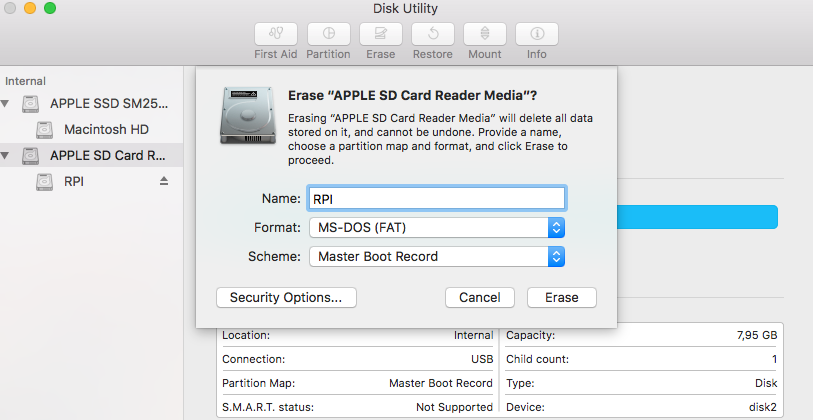
\includegraphics[width=0.7\textwidth]{/Users/allexoliveira/PharoThingsBook/Booklet-APharoThingTutorial/_result/pdf/Chapters/Chap1GettingStarted/figures/pharothings-install-raspberry-pi-raspbian-osx-arm.png}\caption{Preparing SD Card.\label{macInstall}}\end{center}
\end{figure}



\begin{figure}

\begin{center}
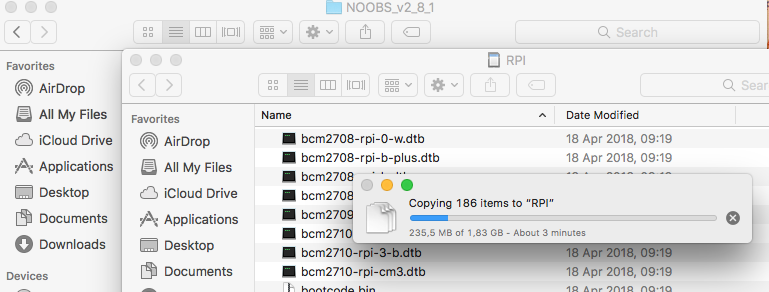
\includegraphics[width=0.7\textwidth]{/Users/allexoliveira/PharoThingsBook/Booklet-APharoThingTutorial/_result/pdf/Chapters/Chap1GettingStarted/figures/pharothings-install-raspberry-pi-raspbian-linux-arm-copy.png}\caption{Copying NOOBS.\label{macCopy}}\end{center}
\end{figure}

\section{Copying Raspbian files on Linux}\section{Copying Raspbian files on Windows}\section{Installing the Raspbian in Raspberry Pi}
Insert the SD Card on Raspberry and turn it on. Select “Raspbian” and “Yes” as shown by Figure \ref{install}.


\begin{figure}

\begin{center}
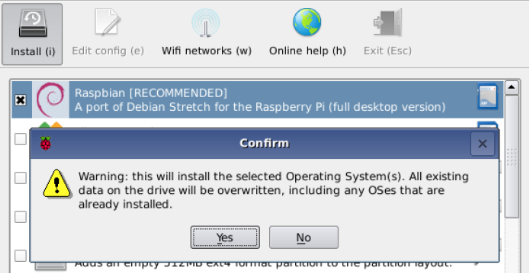
\includegraphics[width=0.6\textwidth]{/Users/allexoliveira/PharoThingsBook/Booklet-APharoThingTutorial/_result/pdf/Chapters/Chap1GettingStarted/figures/pharothings-install-raspberry-pi-raspbian-linux-arm-install.png}\caption{Installing Raspbian.\label{install}}\end{center}
\end{figure}


In a few minutes, you will have your Raspberry Pi running Raspbian OS.
Now you can install PharoThings and control devices remotely. 
\section{Installing PharoThings on Raspberry Pi}
Install PharoThings requires to get Pharo, PharoThings and an ARM virtual machine. We will build the image on our local computer with the correct files and after we will copy to a Raspberry Pi and execute it there. In the third step, we will connect the Pharo from the local computer into Pharo of Raspberry Pi.
\subsection{Download PharoLauncher}
Use the PharoLauncher (an application to help you running multiple versions and images of Pharo) and install Pharo 6.1. You can get the launcher from \url{http://pharo.org/download}.
You can also directly install a version of Pharo from the same place.


\begin{figure}

\begin{center}
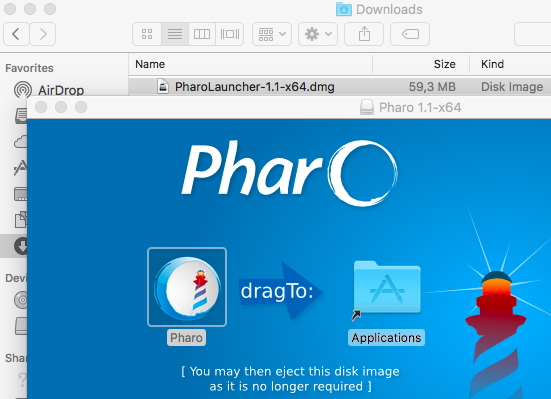
\includegraphics[width=0.6\textwidth]{/Users/allexoliveira/PharoThingsBook/Booklet-APharoThingTutorial/_result/pdf/Chapters/Chap1GettingStarted/figures/InstallLauncher.png}\caption{Installing PharoLauncher.\label{installLauncher}}\end{center}
\end{figure}

\subsection{Download Pharo 61}
Run the Pharo Launcher. Double click the distribution you want to create a image and give a name to image (see Figure \ref{InstallPharo61}). A short name and without spaces is recommended, because we will type this name and path in command line on Linux. 


\begin{figure}

\begin{center}
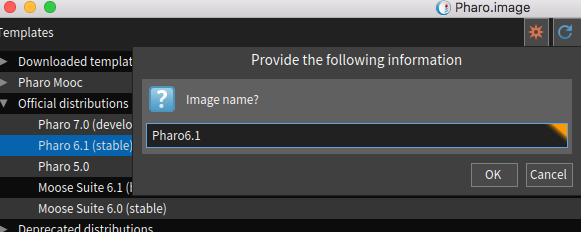
\includegraphics[width=0.6\textwidth]{/Users/allexoliveira/PharoThingsBook/Booklet-APharoThingTutorial/_result/pdf/Chapters/Chap1GettingStarted/figures/Select61.png}\caption{Download Pharo 61.\label{InstallPharo61}}\end{center}
\end{figure}

\subsection{Execute your Pharo image}
Launch the image as shown in Figure \ref{Execute61}. A folder with the image name will be created inside the folder Pharo:  \textcode{/Users/your\_user\_name/Documents/Pharo/}

In this example the folder is  \textcode{/Users/my\_user\_name/Documents/Pharo/Pharo6.1}


\begin{figure}

\begin{center}
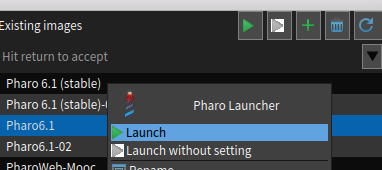
\includegraphics[width=0.6\textwidth]{/Users/allexoliveira/PharoThingsBook/Booklet-APharoThingTutorial/_result/pdf/Chapters/Chap1GettingStarted/figures/Execute61.png}\caption{Open your Pharo image.\label{Execute61}}\end{center}
\end{figure}

\subsection{Load PharoThings}
Open Playground and execute this command to install the server part of PharoThings (as shown in Figure \ref{LoadingPharoThings}):

\begin{displaycode}{plain}
Metacello new
	baseline: 'PharoThings';
	repository: 'github://pharo-iot/PharoThings/src';
	load: #(RemoteDevServer Raspberry).
\end{displaycode}


\begin{figure}

\begin{center}
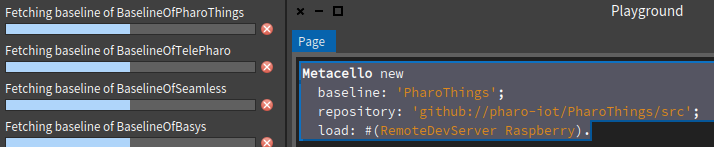
\includegraphics[width=0.6\textwidth]{/Users/allexoliveira/PharoThingsBook/Booklet-APharoThingTutorial/_result/pdf/Chapters/Chap1GettingStarted/figures/LoadingPharoThings.png}\caption{Loading PharoThings.\label{LoadingPharoThings}}\end{center}
\end{figure}


Then configure image to disable slow browser plugins (instead remote browser will be much slower):

\begin{displaycode}{plain}
ClySystemEnvironmentPlugin disableSlowPlugins.
\end{displaycode}
\subsection{Snapshot your Image}
 In Pharo, click and “Save and Quit”. This way all your code and configurations are saved and ready to be reused.
 
 
\subsection{Download the VM}
\begin{itemize}
\item Download ArmVM from \url{http://files.pharo.org/vm/pharo-spur32/linux/armv6/latest.zip}.
\item Unzip it
\item Copy the files shown in FIgure \ref{CopyARM}  to Pharo folder \textcode{/Users/your\_user\_name/Documents/Pharo/pharo\_image\_folder} 
\end{itemize}


\begin{figure}

\begin{center}
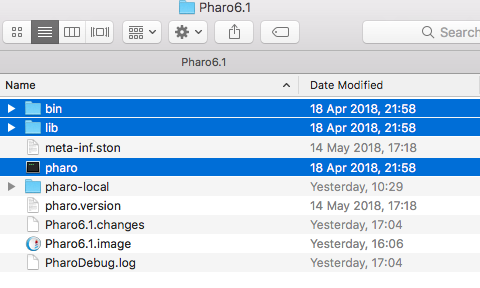
\includegraphics[width=0.6\textwidth]{/Users/allexoliveira/PharoThingsBook/Booklet-APharoThingTutorial/_result/pdf/Chapters/Chap1GettingStarted/figures/CopyARM.png}\caption{Copying PharoARM.\label{CopyARM}}\end{center}
\end{figure}

\subsection{Copying Sources}
Copy the file PharoV60.sources from the folder \textcode{/Applications/Pharo.app/Contents/MacOS} to folder \textcode{/Users/your\_user\_name/Documents/Pharo/images/pharo\_image\_folder/lib/pharo/5.0-201804182009/}
\subsection{Copy to the Raspberry}
Copy this folder to your Raspberry Pi (via flashdrive, network etc). The folder must have the structure shown in Figure \ref{OnRasp}.


\begin{figure}

\begin{center}
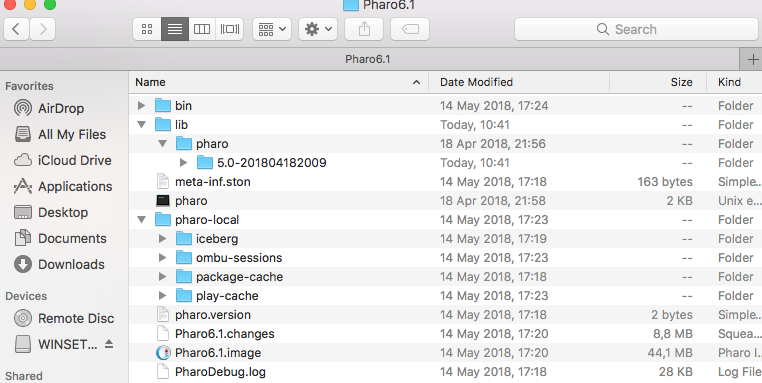
\includegraphics[width=0.6\textwidth]{/Users/allexoliveira/PharoThingsBook/Booklet-APharoThingTutorial/_result/pdf/Chapters/Chap1GettingStarted/figures/OnRasp.png}\caption{Copying the folder on your Raspberry.\label{OnRasp}}\end{center}
\end{figure}

\section{Execute PharoThings on Raspberry}\subsection{Turn on your Raspberry and connect it to the network.}
In this example, the folder Pharo6.1 was copied to folder \textcode{/home/pi/}.

Is necessary apply execute permissions on the Pharo files, using the command chmod +x

\begin{displaycode}{plain}
chmod +x /home/pi/Pharo6.1/pharo

chmod +x /home/pi/Pharo6.1/lib/pharo/5.0-201804182009/pharo
\end{displaycode}
\subsection{Start Server}
Start the Pharo typing the following command in the Terminal on your Raspberry :

\begin{displaycode}{plain}
pharo --headless Server.image remotePharo --startServerOnPort=40423
\end{displaycode}

If all is right, you will see the answer:

\begin{displaycode}{plain}
'a TlpRemoteUIManager is registered on port 40423'
\end{displaycode}

So now we have the Raspberry running the TelePharo on TCP port 40423 (as shown in Figure \ref{Commandline}) and we can connect into it from another computer.


\begin{figure}

\begin{center}
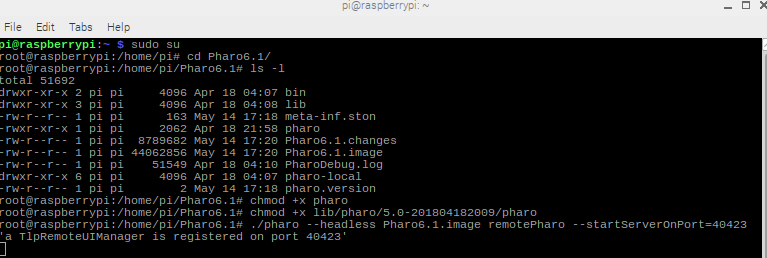
\includegraphics[width=0.6\textwidth]{/Users/allexoliveira/PharoThingsBook/Booklet-APharoThingTutorial/_result/pdf/Chapters/Chap1GettingStarted/figures/Commandline.png}\caption{Server up and running.\label{Commandline}}\end{center}
\end{figure}

\section{Connecting Pharo client on remote Pharo}
Open again the Pharo on your local computer and execute this command to install the PharoThings client:

\begin{displaycode}{plain}
Metacello new
baseline: 'PharoThings';
repository: 'github://pharo-iot/PharoThings/src';
load: 'RemoteDev.
\end{displaycode}

Type this command to connect to the remote TelePharo on Raspberry (change the IP to your Raspberry IP):

\begin{displaycode}{plain}
remotePharo := TlpRemoteIDE connectTo: (TCPAddress ip: #[193 51 236 167] port: 40423)
\end{displaycode}

Here we are using specialized Raspberry tools. They require the auto-refresh feature of inspector which is not enabled by default in Pharo 6. To activate it evaluate:

\begin{displaycode}{plain}
GTInspector enableStepRefresh
\end{displaycode}

So for your board model you need to choose an appropriate board class. For Raspberry, it will be one of the RpiBoard subclasses. Currently, you can use the following classes according to the models:

\begin{itemize}
\item RpiBoardBRev1: Raspberry Pi Model B Revision 1
\item RpiBoardBRev2: Raspberry Pi Model B Revision 2
\item RpiBoard3B: Raspberry Pi Model B+, Pi2 Model B, Pi3 Model B, Pi3 Model B+
\end{itemize}

With the chosen class evaluate the following code to open an inspector:

\begin{displaycode}{plain}
remoteBoard := remotePharo evaluate: [ RpiBoardBRev1 current].
remoteBoard inspect.
\end{displaycode}

And will be open the inspector showing the PIN scheme (as shown in Figure \ref{PharoThingsinspector})


\begin{figure}

\begin{center}
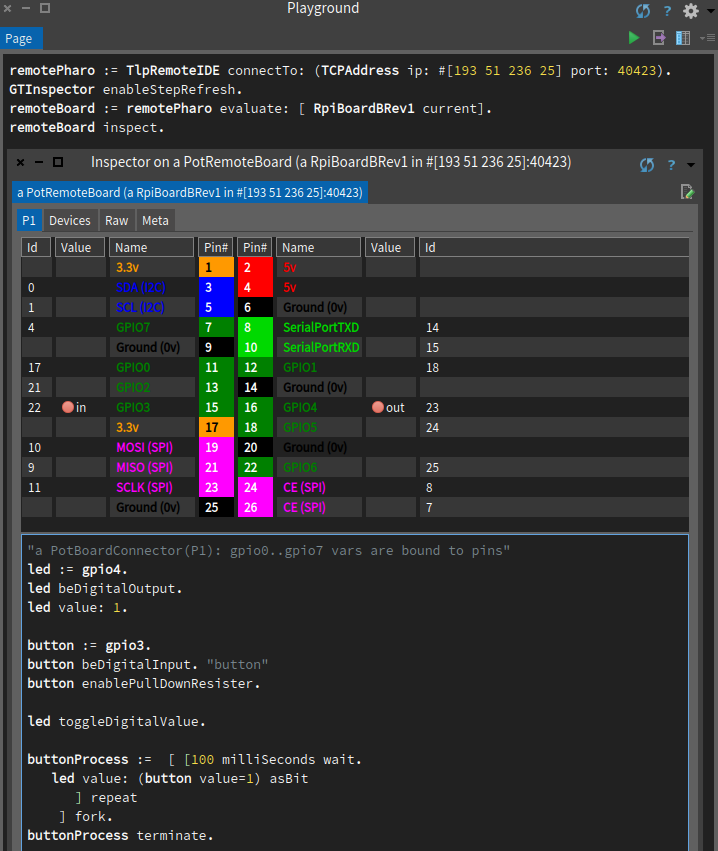
\includegraphics[width=0.6\textwidth]{/Users/allexoliveira/PharoThingsBook/Booklet-APharoThingTutorial/_result/pdf/Chapters/Chap1GettingStarted/figures/PharoThingsInspector.png}\caption{Remote GPIO inspector\label{PharoThingsinspector}}\end{center}
\end{figure}

\subsection{GPIOs}
The board inspector provides a scheme of pins similar to Raspberry Pi docs. But here it is a live tool which represents the current pins state.

In the picture the board is shown with two configured pins: gpio3 and gpio4 which are connected to physical button and led accordingly.

Digital pins are shown with green/red icons which represent high/low (1/0) values. In case of output pins you are able to click on the icon to toggle the value. Icons are updated according to pin value changes. If you click on physical button on your board the inspector will show the updated pin state by changing its icon color.

The evaluation pane in the bottom of the inspector provides bindings to gpio pins which you can script by \#doIt/printIt commands. The example shows expressions which were used to configure a button and led.
\section{In the next chapter}
Now that we have installed the Operation System and PharoThings in the Raspberry Pi, we can play with LEDs, sensors, LCD displays and more. 

In the next chapter we will see how turing on/off a LED using PharoThings. 
\chapter{Lesson 1 – Turning on/off LED }
One of the classic analogies in electronics to “Hello World” is turn on a led or lamp. In this first lesson, we will learn how to connect correctly an LED in your Raspberry Pi and how to use PharoThings to control this led by turning it on and off.

Coding in Pharo is very simple, but it is very powerful and you can control all the GPIOs of your Raspberry Pi remotely.

If you didn’t see how to install the PharoThings on your Raspberry Pi and how to control it remotely, you can find the instructions on Chapter 1.
\section{What we need?}
In this lesson we will use a very simple setup.
\subsection{Components}
\begin{itemize}
\item 1 Raspberry Pi connected to your network (wired or wireless)
\item 1 Breadboard
\item 1 LED
\item 1 Resistor (330ohms)
\item Jumper wires
\end{itemize}
\section{Experimental theory}
Before constructing any circuit, you must know the parameters of the components in the circuit, such as their operating voltage, operating circuit, etc.
\subsection{The LED}
To turn on the LED, we need to send the correct voltage and current to it. The voltage and current can’t be high, otherwise, the led will burn, or in some cases, damage the Raspberry.

Typically, the forward voltage of an LED is between 1.8 and 3.3 volts. It varies by the color of the LED. A red LED typically drops 1.8 volts, but voltage drop normally rises as the light frequency increases, so a blue LED may drop from 3 to 3.3 volts{[}1{]}.

Most 3mm and 5mm LEDs will operate close to their peak brightness at a drive current of 20 mA. This is a conservative current: it doesn’t exceed most ratings (your specs may vary, or you may not have any specs–in this case, 20 mA is a good default guess {[}2{]})

In this experiment, the operating voltage of the LED is between 1.5V and 2.0V and the operating current is between 10mA and 20mA.
\subsection{The Resistor}
We must always use resistors to connect LEDs up to the GPIO pins of the Raspberry Pi to limit the voltage and current between the LED and the Raspberry to a safe value.

A small change in voltage can produce a huge change in current (see more: LED Current vs. Voltage {[}2{]})

In this experiment, we will use a 330ohm resistor. To identify the correct resistor, follow one of the following color sequences, depending on the number of bands {[}3{]}:

\begin{itemize}
\item If there are four colour bands, they will be Orange, Orange, Brown, and then Gold;
\item If there are five bands, then the colours will be Orange, Orange, Black, Black, Brown.
\end{itemize}

It does not matter which way round you connect the resistors (in this experiment). Current flows in both ways through them. This means that you can connect the resistor at the positive pole or the negative pole of the LED, as well as starting with the first or last color, as shown in the Picture \ref{Ledpolarity}.

But the LEDs will only work if the power is supplied correctly (if the polarity is correct). You will not burn the LEDs if they connect the wrong way – they just will not turn on.


\begin{figure}

\begin{center}
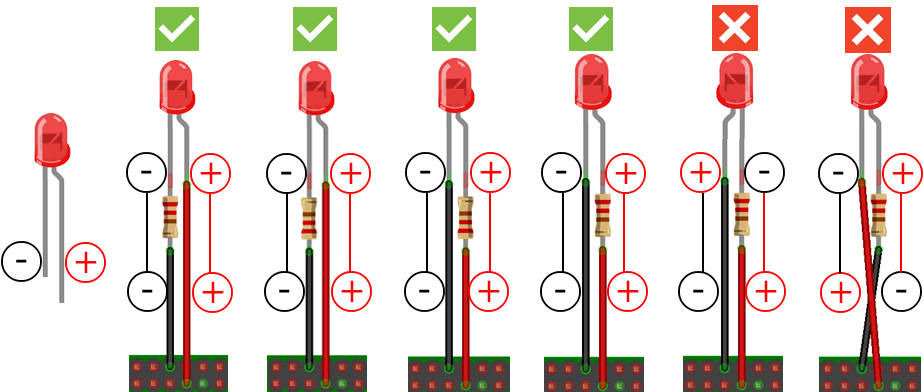
\includegraphics[width=0.6\textwidth]{/Users/allexoliveira/PharoThingsBook/Booklet-APharoThingTutorial/_result/pdf/Chapters/Chap2LED/figures/pharothings-led-polarity-resistors.png}\caption{Led polarity and resistors.\label{Ledpolarity}}\end{center}
\end{figure}

\subsection{The Breadboard}
A breadboard is used to build prototyping of electronics. With a breadboard, it is not necessary to use solder, this way you can reuse the board. This makes it easy to use to create temporary prototypes and experiment with circuit design.

The holes in the breadboard are connected following a pattern, as shown in the Picture \ref{Breadboard}.

\begin{itemize}
\item The red (+) and blue (-) rail are connected horizontally;
\item The holes in the middle are connected vertically.
\end{itemize}


\begin{figure}

\begin{center}
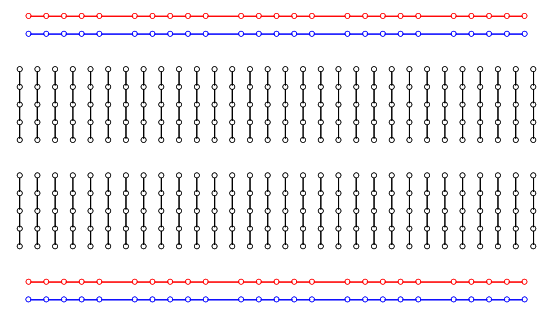
\includegraphics[width=0.6\textwidth]{/Users/allexoliveira/PharoThingsBook/Booklet-APharoThingTutorial/_result/pdf/Chapters/Chap2LED/figures/pharothings-breadboard.png}\caption{Breadboard scheme.\label{Breadboard}}\end{center}
\end{figure}

\section{Experimental procedure}
Now we will build the circuit. This circuit consists of an LED that lights up when power is applied, a resistor to limit current and a power supply (the Rasp).

\begin{itemize}
\item Connect the Ground PIN from Raspberry in the breadboard blue rail (-). Raspeberry Pi models with 40 pins has 8 GPIO ground pins. You can connect with anyone. In this experiment we will use the PIN6 (Ground);
\item Then connect the resistor from the same row on the breadboard to a column on the breadboard, as shown below;
\item Now push the LED legs into the breadboard, with the long leg (with the kink) on the right;
\item And insert a jumper wire connecting the rigth column and the PIN7 (GPIO7).
\end{itemize}

The Figure \ref{physicalLed} shows how the electric connection is made:


\begin{figure}

\begin{center}
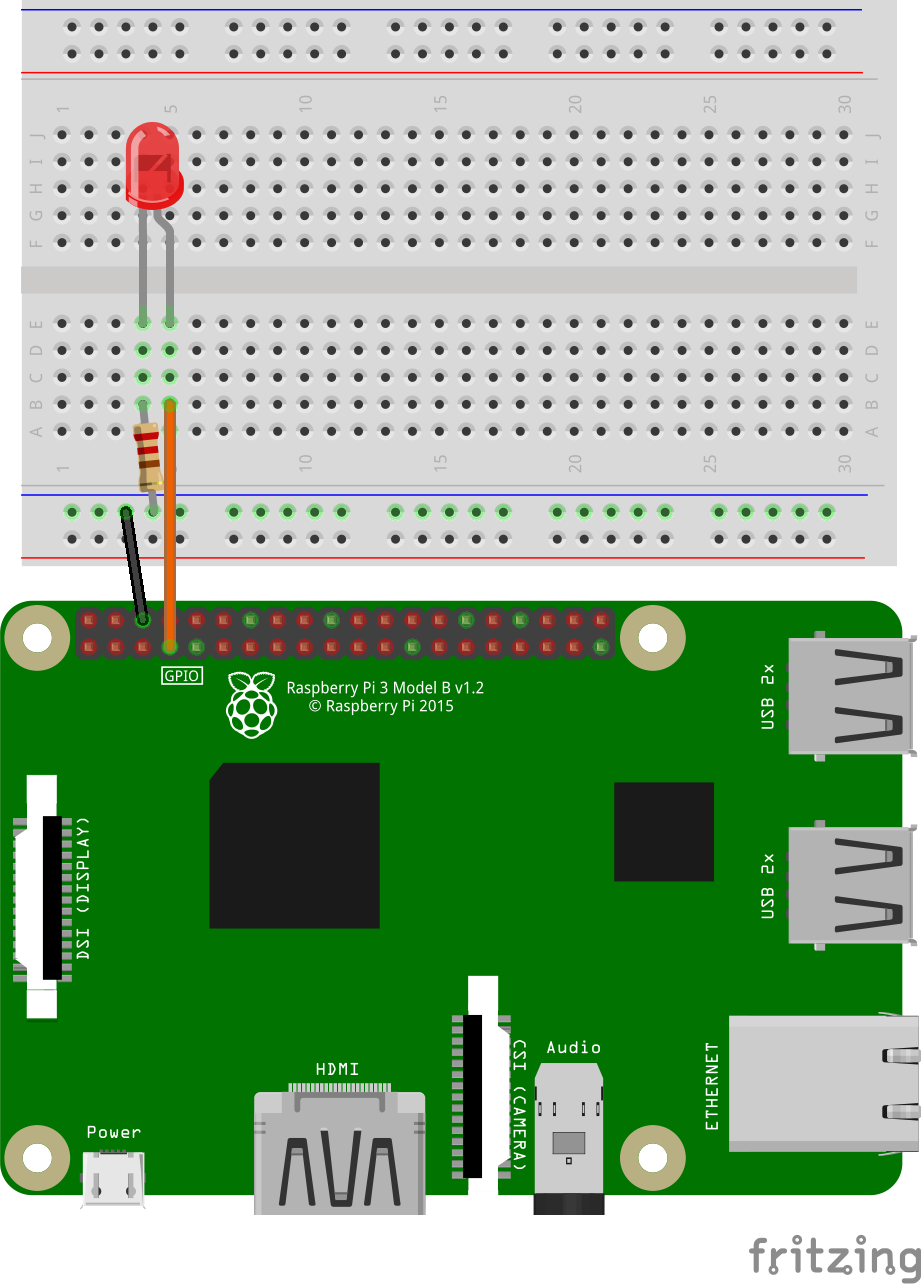
\includegraphics[width=0.6\textwidth]{/Users/allexoliveira/PharoThingsBook/Booklet-APharoThingTutorial/_result/pdf/Chapters/Chap2LED/figures/pharothings-raspberry-led-resistor-lesson-01.png}\caption{Physical connection LED.\label{physicalLed}}\end{center}
\end{figure}

\section{Experimental code}
Now, we can write some code in Pharo to control the GPIOs using PharoThings and turn the LED on. We have 2 options to do this:

\begin{itemize}
\item Write the code locally on the Raspberry;
\item Use TelePharo to connect from your computer into the Raspberry and do all the work remotely.
\end{itemize}

In this experiment, we will use the second option: connect and do all the work remotely. 

If you didn’t see how to install the PharoThings on your Raspberry Pi and how to control it remotely, take a look in the Chapter 1: Instalattions.
\subsection{Connecting remotely}
Through your local Pharo image, let's connect in the Pharo image running on Raspberry, enable the auto-refresh feature of the inspector and open the inspector. Run this code in your local playground:

\begin{displaycode}{plain}
remotePharo := TlpRemoteIDE connectTo: (TCPAddress ip: #[193 51 236 167] port: 40423)
GTInspector enableStepRefresh
remoteBoard := remotePharo evaluate: [ RpiBoardBRev1 current].
remoteBoard inspect.
\end{displaycode}

In your inspect window (Inspector on a PotRemoteBoard) you can see a scheme of pins similar to Raspberry Pi docs. But here it is a live tool which represents the current pins state{[}4{]}.


\begin{figure}

\begin{center}
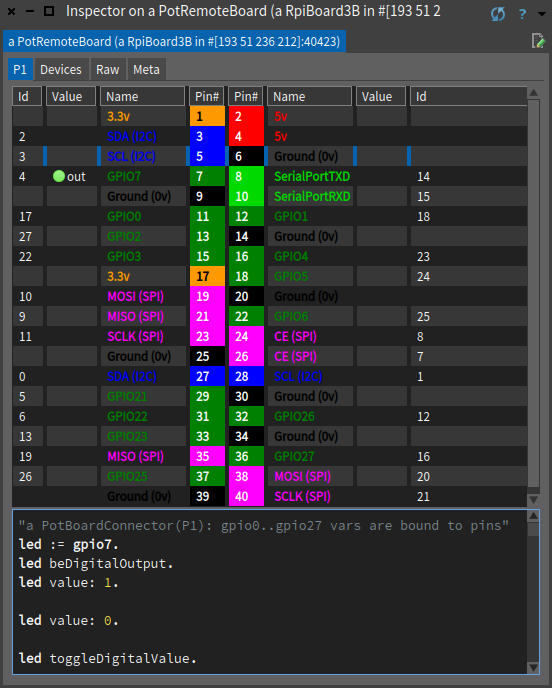
\includegraphics[width=0.6\textwidth]{/Users/allexoliveira/PharoThingsBook/Booklet-APharoThingTutorial/_result/pdf/Chapters/Chap2LED/figures/pharothings-inspector-remote-board-raspberry.png}\caption{Remote Board Inspector.\label{remoteBoard}}\end{center}
\end{figure}


Digital pins are shown with green/red icons which represent high/low (1/0) values. In case of output pins you are able to click on the icon to toggle the value.

For control the led we first introduced named variable \#led which we assigned to GPIO7 pin instance:

\begin{displaycode}{plain}
led := gpio7.
\end{displaycode}

Then we configured the pin to be in digital output mode and set the value:

\begin{displaycode}{plain}
led beDigitalOutput.
led value: 1.
\end{displaycode}

It turned the led on.

You can notice that gpio variables are not just numbers/ids. PharoThings models boards with first class pins. They are real objects with behaviour. For example you can ask pin to toggle a value:

\begin{displaycode}{plain}
led toggleDigitalValue.
\end{displaycode}

Or ask a pin for current value if you want to check it:

\begin{displaycode}{plain}
led value.
\end{displaycode}
\section{What did we learn?}
With PharoThings you can remotely control all the GPIOs in your running board!

You can:

\begin{itemize}
\item Interact remotely with pins and boards;
\item See the current pins state in real time;
\item Run the code dynamically.
\item Easy, powerful.
\end{itemize}
\section{In the next lesson}
Let’s use what we learned in this lesson and write a simple code to blink the LED.
\chapter{Lesson 2 – Blinking LED }
Now we can play with the LEDs, turn them on and off. Let's use this basic setup to write some code on the inspector playground to blink the LED. Next, we will learn how to remotely create a very simple application using classes, methods, and instances to control the LED.
\section{What we need?}
We are using the same last lesson setup: 1 Raspberry Pi, 1 Breadboard, 1 LED, 1 Resistor 330ohms. If you didn't do the last lesson to understand how to do the connections, go back to Chapter 2 and do it.
\subsection{Connecting remotely}
Through your local Pharo image, let's connect in the Pharo image by running on Raspberry, enable the auto-refresh feature of the inspector, and open the inspector.

Run this code in your local playground:

\begin{displaycode}{plain}
remotePharo := TlpRemoteIDE connectTo: (TCPAddress ip: #[193 51 236 212] port: 40423)
GTInspector enableStepRefresh.
remoteBoard := remotePharo evaluate: [ RpiBoardBRev1 current].
remoteBoard inspect.
\end{displaycode}
\section{Experimental code}
In your inspect window (Inspector on a PotRemoteBoard), let's initialize the led and set the pin 7 to be in digital output mode as we did in the last lesson:

\begin{displaycode}{plain}
led := gpio7.
led beDigitalOutput.
\end{displaycode}

To blink the LED let's create a simple loop to change the value of the LED every 1 second by 10 times. To change the value of the object (led value), let's call the method \textcode{toggleDigitalValue}, as we saw previously:

\begin{displaycode}{plain}
[ 10 timesRepeat: [
	led toggleDigitalValue.
 	(Delay forSeconds: 1) wait
] ] forkNamed: 'BlinkerProcess'.
\end{displaycode}

Run this code, as shown in Figure \ref{RemoteInspector} and... \textcode{cool}! Now your LED is blinking!


\begin{figure}

\begin{center}
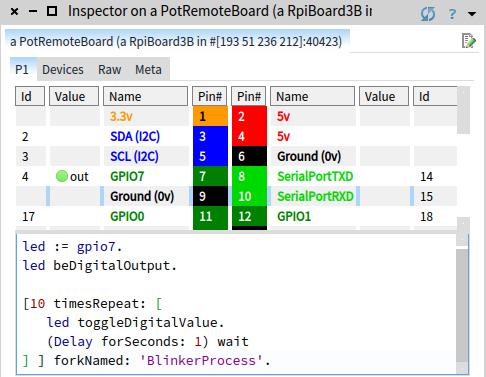
\includegraphics[width=0.7\textwidth]{/Users/allexoliveira/PharoThingsBook/Booklet-APharoThingTutorial/_result/pdf/Chapters/Chap3BlinkingLED/figures/pharothings-board-inspector-blink-led.png}\caption{Remote playground.\label{RemoteInspector}}\end{center}
\end{figure}


Change the values to repeat more times and to wait less time between toggling. This will cause the LED to blink faster.
\section{In the next lesson}
In this tutorial, you learned how to blink a LED by typing some code in the remote inspector. But with Pharo we can do more! Pharo is a new generation reflective language and programming environment. And in the next lesson, let’s start using object-oriented programming, OOP. Let's create a simple application, writing classes and methods, all remotely.
\chapter{A brief introduction to Pharo object-oriented language}
Pharo is a new generation reflective language and programming environment. The last code was executed inside the remote inspector. To get started using OOP (Object-oriented programming) with classes, methods, and instances, I invite you to implement a simple application to blink the LEDs.
Pharo will fundamentally change your perception about what OOP is.
\section{Developing a simple LED blinker}
The following part of this chapter and application was based on the exercise \textcode{Developing a Simple Counter}, of Week 1 of Pharo MOOC (https://mooc.pharo.org/). I strongly recommend that you read and do the \symbol{34}counter exercise\symbol{34} to better understand the concepts explained here. And, of course, do the MOOC to learn how to develop using Pharo and the OOP concept, Object-oriented programming.
\section{Our use case}
We want to create a blinker led using a few parameters such as time to repeat the blinking LED and how many seconds to wait between blinks. The following code should run in the playground when we finish this lesson:

\begin{displaycode}{plain}
|blinker|
blinker := Blinker new.
blinker timesRepeat: 10 waitForSeconds: 1.
\end{displaycode}

Here is a short explanation of this code:

\begin{itemize}
\item In the first line, we declare the variable \textcode{blinker}. We can use any name. We will use this variable to create an object using the Blinker class;
\item In the second line, we instantiate the Blinker class (with uppercase B) in the \textcode{blinker} variable, creating an object. In this lesson, we will create this class and methods to control the LED;
\item In the third line, we send some messages to \textcode{blinker} object, for how long and how many times per second. This will make the GPIO behave according to the parameters sent.
\end{itemize}

Now we will develop all the mandatory class and methods to support this scenario.
\section{Create your own class remotely}
Let's create our first class. To create a class in Pharo, we need first to create a package. Inside the package, you can create many classes and inside the classes, you can create many methods. The methods are organized in protocols, to become more easily navigate between them. Take a look in Figure \ref{RemoteBrowser} to better understanding. *edit image, put name in windows

In your local playground, call the Remote System Browser of your Raspberry Pi. If you are already connected in your Raspberry Pharo, you do not need to run the first line below again. This will open a window as shown in Figure \ref{RemoteBrowser} 


\begin{figure}

\begin{center}
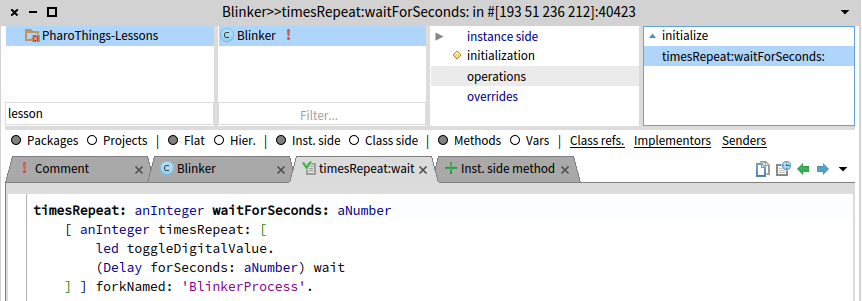
\includegraphics[width=1.0\textwidth]{/Users/allexoliveira/PharoThingsBook/Booklet-APharoThingTutorial/_result/pdf/Chapters/Chap4IntroductiontoPharoOOP/figures/pharothings-remote-system-browser.png}\caption{Remote System Browser.\label{RemoteBrowser}}\end{center}
\end{figure}


\begin{displaycode}{plain}
remotePharo := TlpRemoteIDE connectTo: (TCPAddress ip: #[193 51 236 212] port: 40423).
remotePharo openBrowser.
\end{displaycode}
\section{Create a package}
Let's create a package using the Remote Browser. Right-click the package area and enter the package name, as shown in Figure \ref{CreatingPackage}. In this example, we will create a package named \textcode{PharoThings-Lessons}.


\begin{figure}

\begin{center}
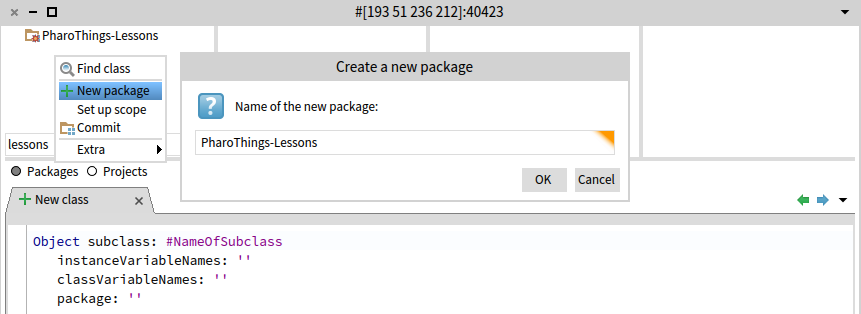
\includegraphics[width=1.0\textwidth]{/Users/allexoliveira/PharoThingsBook/Booklet-APharoThingTutorial/_result/pdf/Chapters/Chap4IntroductiontoPharoOOP/figures/pharothings-creating-package.png}\caption{Creating a package remotely.\label{CreatingPackage}}\end{center}
\end{figure}

\section{Create a class}
To create a new class, edit the default class template by changing the \#NameOfSubclass to the name of the new class. In this example let's create the class \textcode{\#Blinker}. Take care that the class name begins with a capital letter and that you do not remove the octothorpe symbol (\#) in front of NameOfSubClass. 

You must then fill in the names of the instance variables for this class. We need an instance variable called \textcode{led}. Be careful to leave the strings quotes!

\begin{displaycode}{plain}
Object subclass: #Blinker
  instanceVariableNames: 'led'
  classVariableNames: ''
  package: 'PharoThings-Lessons'
\end{displaycode}

Now we need to compile it. Right click on the code area and select Accept option. The \textcode{Blinker} class is now compiled and added to the system, as shown in Figure \ref{CreatingClass}.


\begin{figure}

\begin{center}
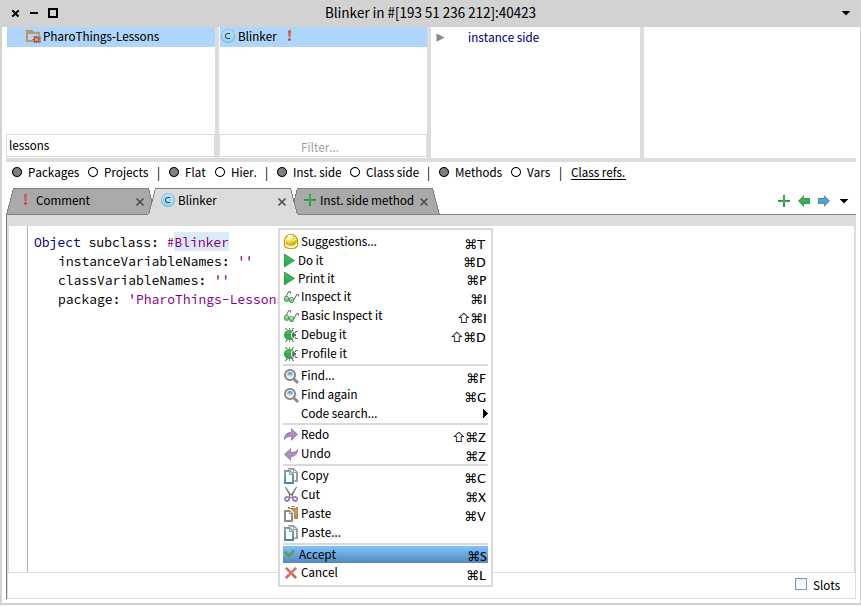
\includegraphics[width=1.0\textwidth]{/Users/allexoliveira/PharoThingsBook/Booklet-APharoThingTutorial/_result/pdf/Chapters/Chap4IntroductiontoPharoOOP/figures/pharothings-creating-class}\caption{Creating a class remotely.\label{CreatingClass}}\end{center}
\end{figure}

\section{Create a protocol}
Let's create a new protocol to organize the methods. The first protocol we are going to create is \textcode{initialization}, as shown in Figure \ref{CreatingProtocol}.


\begin{figure}

\begin{center}
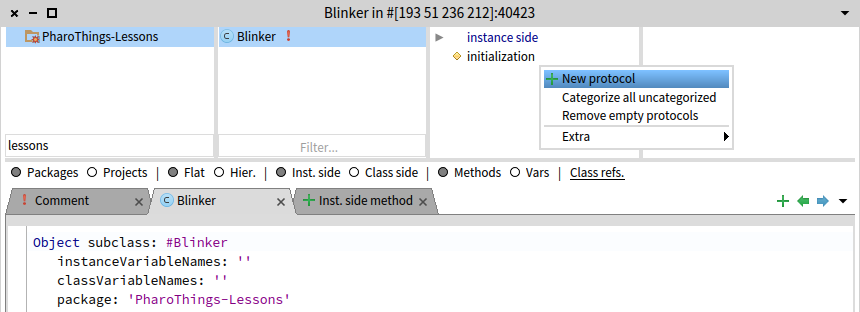
\includegraphics[width=1.0\textwidth]{/Users/allexoliveira/PharoThingsBook/Booklet-APharoThingTutorial/_result/pdf/Chapters/Chap4IntroductiontoPharoOOP/figures/pharothings-creating-protocol}\caption{Creating a package remotely.\label{CreatingProtocol}}\end{center}
\end{figure}

\section{Creating an initialize method}
Inside this protocol, we will create a \textcode{initialize} method. This means that every time we create a new object using this class, in this case, the Blinker class, this method will be executed to define some parameters in the new object.

Let's use the instance variable \textcode{led}, which we defined when we created the class. The instance variable is private to the object and accessible by any methods inside this class. These methods can access this variable to get or set any value to it.

\begin{displaycode}{plain}
initialize 
  led := PotClockGPIOPin id: 4 number: 7. 
  led board: RpiBoard3B new; beDigitalOutput
\end{displaycode}

Here is a short explanation of this code:

\begin{itemize}
\item The first line defines the name of the method;
\item In the second line, we configure the GPIO that we wanna use. Note that we need the GPIO number and ID. The ID is required to communicate with Wiring Pi Library. You can see the \textcode{ID} and \textcode{GPIO number} in PotRemoteBoard inspector, as shown in Figure \ref{RemoteInspector};
\item In the third line, we define the model of the Raspberry board and configure this GPIO as beDigitalOutput. This means that when the GPIO change to value:1, the power will go out of the GPIO to power the LED.
\end{itemize}


\begin{figure}

\begin{center}
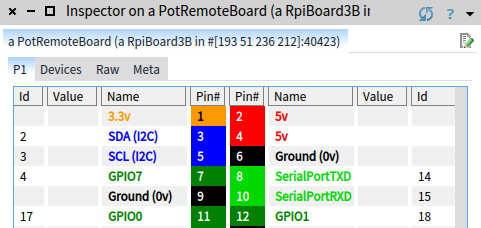
\includegraphics[width=0.7\textwidth]{/Users/allexoliveira/PharoThingsBook/Booklet-APharoThingTutorial/_result/pdf/Chapters/Chap4IntroductiontoPharoOOP/figures/pharothings-board-inspector-id-number.png}\caption{Looking for ID and GPIO number on Remote Inspector.\label{RemoteInspector}}\end{center}
\end{figure}


Compile your code (cmd + S) and the method will be shown in the remote browser, as shown in Figure \ref{InitializeMethod}:


\begin{figure}

\begin{center}
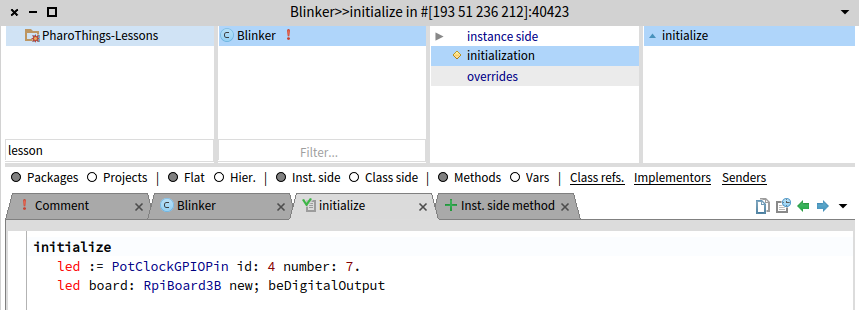
\includegraphics[width=1.0\textwidth]{/Users/allexoliveira/PharoThingsBook/Booklet-APharoThingTutorial/_result/pdf/Chapters/Chap4IntroductiontoPharoOOP/figures/pharothings-creating-method-initialize.png}\caption{Creating a initialize method.\label{InitializeMethod}}\end{center}
\end{figure}

\subsection{Creating a method to do actions}
Now let's create a method to control the object led inside the class Blinker. Let's take the code that we used in PotRemoteBoard inspector to do the LED to blink and replace the numbers on code for two arguments. Create the protocol \textcode{operations} and inside this protocol, create the following method:

\begin{displaycode}{plain}
timesRepeat: anInteger waitForSeconds: aNumber
    [ anInteger timesRepeat: [  
        led toggleDigitalValue. 
        (Delay forSeconds: aNumber) wait  
    ] ] forkNamed: 'BlinkerProcess'.
\end{displaycode}

Here is a short explanation of this code:

\begin{itemize}
\item In the first line, we define the message with timesRepeat: and waitForSeconds:. We inform the kind of value will be received, creating 2 variables: aNumber and anInteger;
\item We replace these variables in the code and now we have the control to say how many times repeat and for how many seconds;
\item We finished the code by putting everything inside a fork to create a process in Pharo. While the process is running, you can open the Remote Process Browser (remotePharo openProcessBrowser) and see the process. This is useful when you wanna kill the remote process.
\end{itemize}

Compile your code (cmd + S) and  the method will be shown in the remote browser, as shown in Figure \ref{OperationsMethod}:


\begin{figure}

\begin{center}
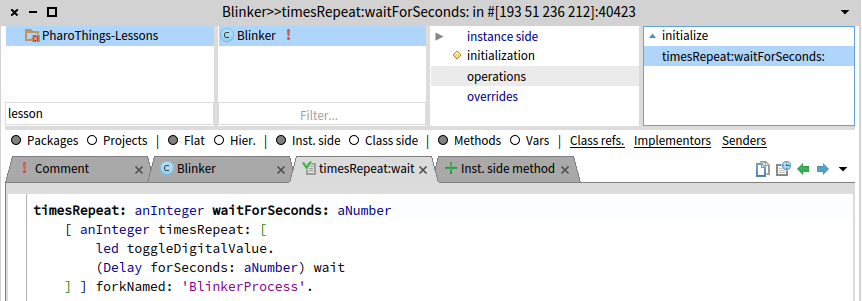
\includegraphics[width=1.0\textwidth]{/Users/allexoliveira/PharoThingsBook/Booklet-APharoThingTutorial/_result/pdf/Chapters/Chap4IntroductiontoPharoOOP/figures/pharothings-creating-method-operations.png}\caption{Creating an operation method.\label{OperationsMethod}}\end{center}
\end{figure}

\section{Using your new class}
Now we can use the class that we created, the Blinker class. To do this, let's open the Remote Playground:

\begin{displaycode}{plain}
remotePharo openPlayground.
\end{displaycode}

and run the code that we saw in the begin of this lesson:

\begin{displaycode}{plain}
|blinker|
blinker := Blinker new. 
blinker timesRepeat: 10 waitForSeconds: 1.
\end{displaycode}

Run this code, as shown in Figure \ref{RemotePlayground} and... \textcode{cool}! Now your LED is blinking! And the better, you did this using object-oriented programming! 

This is very cool, you do not need to change your code every time you wanna change these parameters. Just change the messages you send to the object and it will behave as you want.


\begin{figure}

\begin{center}
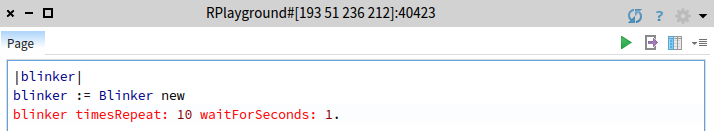
\includegraphics[width=1.0\textwidth]{/Users/allexoliveira/PharoThingsBook/Booklet-APharoThingTutorial/_result/pdf/Chapters/Chap4IntroductiontoPharoOOP/figures/pharothings-remote-playground-blinker.png}\caption{Remote playground.\label{RemotePlayground}}\end{center}
\end{figure}

\section{Save your work}
Don't forget to save your work remotely. To do this, run this command on your local playground:

\begin{displaycode}{plain}
remotePharo saveImage.
\end{displaycode}
\section{Conclusion}
In this tutorial, you learned how to define packages, classes, and methods. The flow of programming that we chose for this first tutorial is similar to most of the programming languages.

With PharoThings you can remotely develop and manage your Raspberry GPIOs. Very easy and powerful.

In the next lesson, let’s use what we learned in this lesson and write a simple code to flow lights using 8 LEDs.
\chapter{Lesson 3 - LED Flowing Lights}
Now we can play with the LEDs, turn them on, off, and blink. Let's put 8 LEDs on the breadboard and create a code to turn on/off one at a time. As we did in the last lesson, let's write the first code in playground and then create a class with methods to better control the flow of LED lights.
\section{What we need?}
We are using the lesson 1 setup, but let's use 8 LEDs and 8 resistors.
\subsection{Components}
\begin{itemize}
\item 1 Raspberry Pi connected to your network (wired or wireless)
\item 1 Breadboard
\item 8 LEDs
\item 8 Resistors 330ohms
\item Jumper wires
\end{itemize}
\section{Experimental procedure}
We saw in the lesson 1 how to connect the LED and resistors on the breadboard. Now let's do the same, but putting more 7 LEDs and resistors on the breadboard.

\begin{itemize}
\item Connect the Ground PIN from Raspberry in the breadboard blue rail (-). 
\item Then connect the 8 resistors from the blue rail (-) to a column on the breadboard, as shown below;
\item Now push the LED legs into the breadboard, with the long leg (with the kink) on the right;
\item And insert the jumper wires connecting the rigth column of each LED to GPIO from 0 to 7, as shown in the Picture \ref{Physical8Leds}.
\end{itemize}

The Figure \ref{Physical8Leds} shows how the electric connection is made:


\begin{figure}

\begin{center}
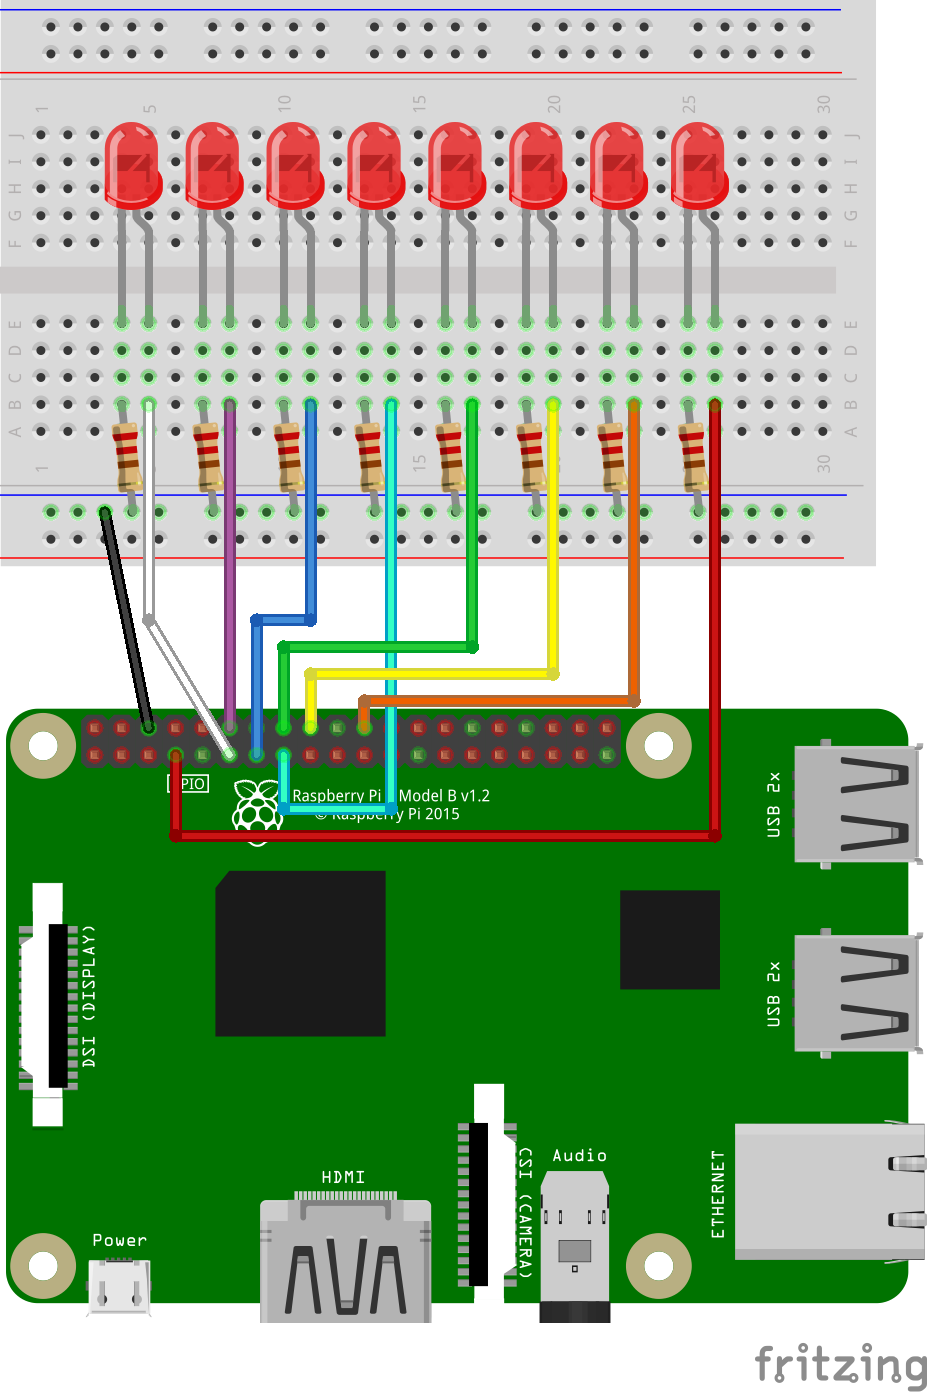
\includegraphics[width=0.6\textwidth]{/Users/allexoliveira/PharoThingsBook/Booklet-APharoThingTutorial/_result/pdf/Chapters/Chap5LEDFlowingLights/figures/pharothings-raspberry-8leds-8resistors-lesson-01.png}\caption{Physical connection 8 LEDs.\label{Physical8Leds}}\end{center}
\end{figure}

\subsection{Connecting remotely}
Through your local Pharo image, let's connect in the Pharo image by running on Raspberry, enable the auto-refresh feature of the inspector, and open the inspector.

Run this code in your local playground:

\begin{displaycode}{plain}
remotePharo := TlpRemoteIDE connectTo: (TCPAddress ip: #[193 51 236 212] port: 40423)
GTInspector enableStepRefresh.
remoteBoard := remotePharo evaluate: [ RpiBoardBRev1 current].
remoteBoard inspect.
\end{displaycode}
\section{Experimental code}
In your inspect window (Inspector on a PotRemoteBoard), let's initialize the 8 LEDs and set the GPIOs to be in digital output mode:

\begin{displaycode}{plain}
code...
\end{displaycode}

To blink the LED let's create a simple loop to change the value of the LED every 1 second by 10 times. To change the value of the object (led value), let's call the method \textcode{toggleDigitalValue}, as we saw previously:

\begin{displaycode}{plain}
code...
\end{displaycode}


% lulu requires an empty page at the end. That's why I'm using
% \backmatter here.
\backmatter

% Index would go here

\end{document}
